% Chapter 6: The Attack Key as Emergent State
% Two Generals Protocol Paper (v2)

The three-phase protocol ($C \rightarrow D \rightarrow T$) does not culminate in a ``decision point'' where a party chooses to attack. Instead, the \emph{attack key} is an emergent state---it either exists or it does not, and both parties can locally determine which.

\subsection{The Attack Key Construction}

\begin{definition}[Attack Key]
The attack key is a tripartite construction requiring:
\begin{enumerate}
    \item Virtual artifact $V$ (emerges when $D_A \land D_B$)
    \item Alice's response (requires $V$ and Alice having $D_B$)
    \item Bob's response (requires $V$ and Bob having $D_A$)
\end{enumerate}
The attack key exists if and only if \emph{all three} components exist.
\end{definition}

In Lean 4:
\begin{verbatim}
def attack_key_emerges (v : Option V) (alice_resp bob_resp : Option Response) :
    Option AttackKey :=
  match v, alice_resp, bob_resp with
  | some v', some a, some b => some (mk_attack_key v' a b)
  | _, _, _ => none
\end{verbatim}

\subsection{Why There Is No Decision}

Traditional protocols have a ``decision point''---a moment where a party commits to an action based on received messages. This creates the classic impossibility: any decision based on message receipt can be undermined by dropping that message.

TGP inverts this. The attack key is not a decision; it is a \emph{mathematical fact} about the state of the world:

\begin{center}
\fbox{
\begin{minipage}{0.85\columnwidth}
\textbf{Attack key exists} if and only if:
\begin{enumerate}
    \item Both parties received both commitments ($C_A$ and $C_B$)
    \item Both parties received both double proofs ($D_A$ and $D_B$)
    \item Both parties created and could exchange triple proofs ($T_A$ and $T_B$)
\end{enumerate}
\end{minipage}
}
\end{center}

Each party can \emph{locally compute} whether the attack key exists by examining what they have received. The bilateral construction property guarantees their computations agree.

\subsection{Local Detectability}

\begin{theorem}[Local Views Agree]
\label{thm:local-views}
If both parties execute the TGP protocol under any adversary, their local inferences about the attack key's existence agree.
\end{theorem}

This is proven exhaustively in Lean 4 via \texttt{channel\_bilateral\_determination}: all 256 possible channel states yield symmetric outcomes. The proof uses \texttt{native\_decide} for complete case coverage.

\subsection{The Knot, Not The Chain}

Traditional acknowledgment protocols create a chain:
\[
\text{MSG} \rightarrow \text{ACK} \rightarrow \text{ACK-of-ACK} \rightarrow \cdots
\]

Every link could be ``the last message'' that fails. TGP creates a \emph{knot}:

\begin{center}
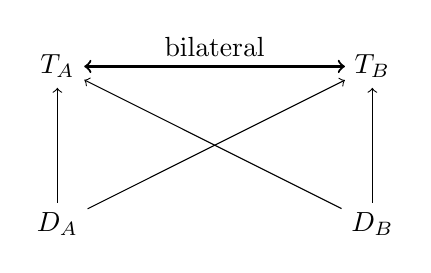
\begin{tikzpicture}[node distance=2cm]
\node (TA) {$T_A$};
\node (TB) [right of=TA, xshift=2cm] {$T_B$};
\draw[<->, thick] (TA) -- (TB) node[midway, above] {bilateral};
\node (DA) [below of=TA] {$D_A$};
\node (DB) [below of=TB] {$D_B$};
\draw[->] (DA) -- (TA);
\draw[->] (DB) -- (TB);
\draw[->] (DA) -- (TB);
\draw[->] (DB) -- (TA);
\end{tikzpicture}
\end{center}

$T_A$ embeds $D_B$; $T_B$ embeds $D_A$. Neither can exist without the other being constructible. There is no ``last message''---there is mutual cryptographic entanglement.

\subsection{The Outcome Table}

Under all possible adversary behaviors, outcomes are symmetric:

\begin{center}
\begin{tabular}{lc}
\toprule
Adversary Behavior & TGP Outcome \\
\midrule
NoChannel (total loss) & CoordinatedAbort \\
Partial delivery & CoordinatedAbort \\
Full delivery (fair-lossy) & CoordinatedAttack \\
Asymmetric channel & CoordinatedAbort \\
\bottomrule
\end{tabular}
\end{center}

Gray said symmetric outcomes are impossible. TGP proves they are guaranteed.
